\section{Results}

After following the approach discussed above, I was able to achieve \textbf{98\% accuracy on the test dataset}.

Below is the \textit{classfication report} of the trained model

\begin{figure}[h]
	\centering
	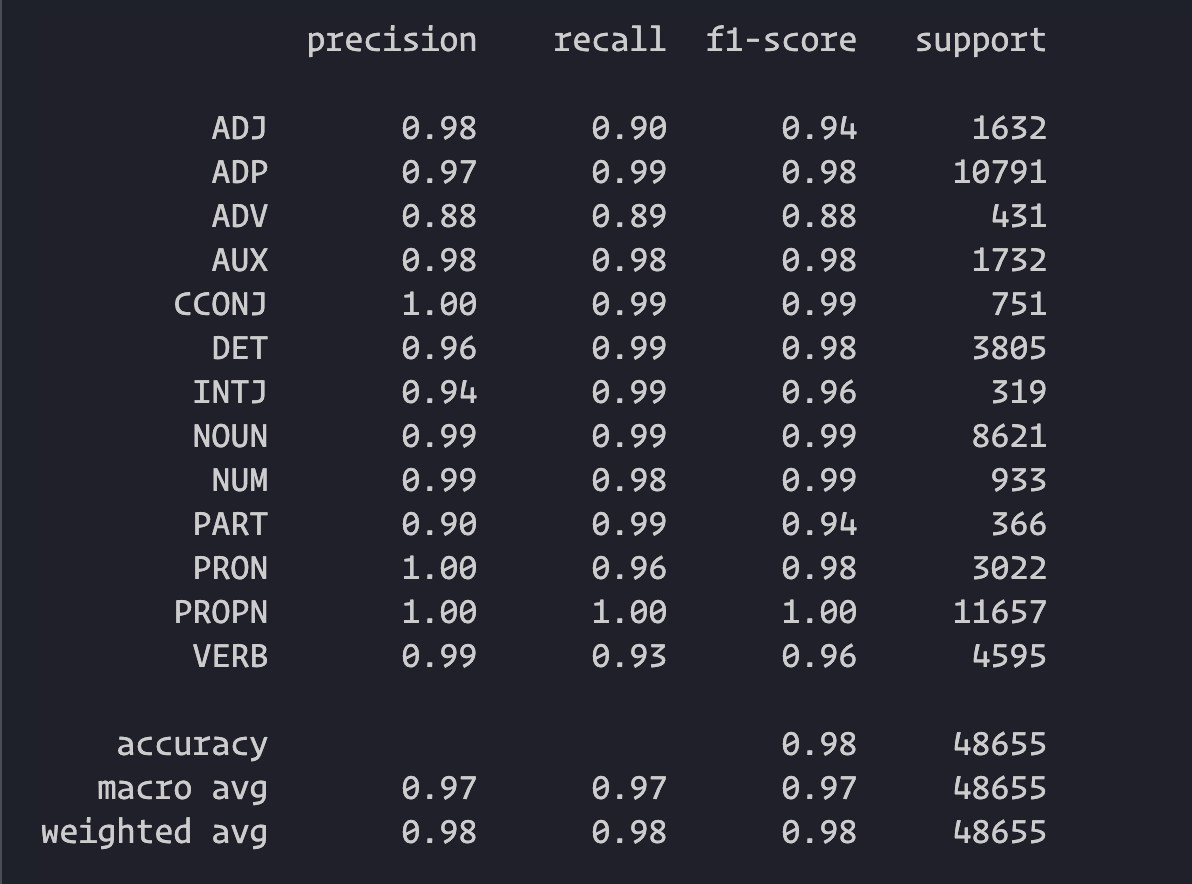
\includegraphics[scale=0.8]{img/class_report.png}
	\caption{Classification Report}
\end{figure}

The figures above depict various metrics such as \textit{precision, recall, and F1-score}, which provide a balance between precision and recall by computing their harmonic mean.


The below plots display the training and validation accuracy, as well as the loss during the training process. These plots provide an analysis of the model's performance with each epoch during training.


\begin{figure}[h]
	\centering
	\subfloat[Train Set Accuracy]{{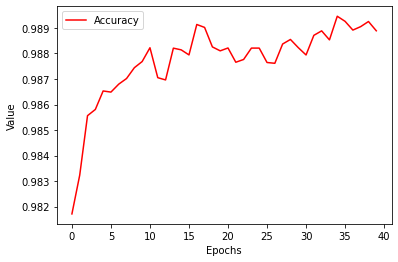
\includegraphics[]{img/train_acc.png} }}
    \qquad
    \subfloat[Train Set Loss]{{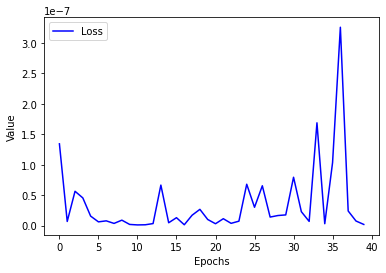
\includegraphics[]{img/train_loss.png} }}
    \caption{Train Set Metrics}
\end{figure}

\begin{figure}[h]
	\subfloat[Validation Set Accuracy]{{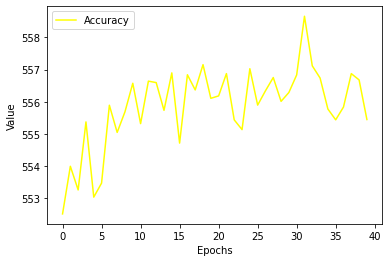
\includegraphics{img/valid_acc.png} }}
    \qquad
    \subfloat[Validation Set Loss]{{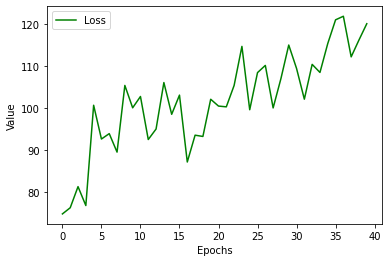
\includegraphics{img/valid_loss.png}}}
    \caption{Validation Set Metrics}
    
    The results demonstrate that as the number of epochs increase, there is a reduction in overall loss and an increase in accuracy. This indicates that the model has been effectively trained.
\end{figure}

    

